\documentclass[12pt]{article}

\usepackage[utf8]{inputenc}
\usepackage[T1]{fontenc}
\usepackage[ngerman]{babel}
\usepackage{amsmath}
\usepackage{graphicx}
\usepackage{setspace}
\usepackage{geometry}
\usepackage{layout}
\usepackage{blindtext}
\usepackage{fancyhdr}
\usepackage{quotes}
\usepackage{csquotes}
\usepackage{times}
%
% For alternative styles, see the biblatex manual:
% http://mirrors.ctan.org/macros/latex/contrib/biblatex/doc/biblatex.pdf
%
% The 'verbose' family of styles produces full citations in footnotes, 
% with and a variety of options for ibidem abbreviations.
%
\usepackage[style=ext-verbose-ibid,backend=biber]{biblatex}

% Include hyperref last
\usepackage{hyperref}
\hypersetup{
    colorlinks=true,
    linkcolor=blue,
    citecolor=blue,
    filecolor=magenta,      
    urlcolor=cyan,
    pdfpagemode=FullScreen,
}
    
\bibliography{sources}

% Bibtext online sources
\DefineBibliographyStrings{german}{
    urlseen = {aufgerufen am},
}

% The following two lines are what needs to be added %
\setcounter{biburllcpenalty}{7000}
\setcounter{biburlucpenalty}{8000}

% Configure the pages
\pagestyle{fancy}
\fancyhf{}
\renewcommand{\headrulewidth}{0mm}
\fancyfoot[R]{\thepage}

\geometry{
 a4paper,
 total={155mm,245mm},
 left=35mm,
 top=25mm,
}
\onehalfspacing

% Titlepage information
\title{Facharbeit}
\author{Jane Doe}
\date{November 2022}

% Do not indent paragraphs
\setlength{\parindent}{0em}

% erst Nachname, dann Vorname
\DeclareNameAlias{default}{family-given}

% Begin main document
\begin{document}

% No dots in toc
\makeatletter
\renewcommand\@dotsep{250}
\makeatother

% Show the current layout
%\layout*

% Hide the page number for title and toc
\addtocontents{toc}{\protect\thispagestyle{empty}}
\pagenumbering{gobble}
\newgeometry{}
\begin{titlepage}
	\centering
	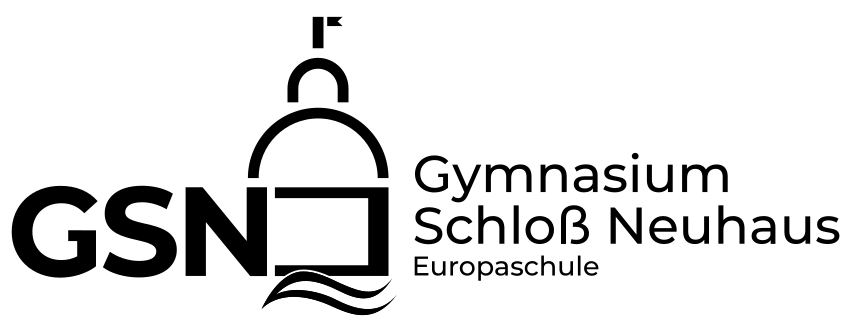
\includegraphics[width=0.4\textwidth]{logo.png}\par\vspace{1cm}
    \begin{bfseries}
	   {\LARGE Gymnasium Schloß Neuhaus \par}
        \large Paderborn \par
    \end{bfseries}
	\vspace{1cm}
	{\huge\bfseries Hier kommt der Titel hin\par}
	\vspace{4cm}
    \begin{flushleft}
    \begin{Large}
        
    Facharbeit im Superkurs \par
    \vspace{1cm}
    \begin{bfseries}
    von
    \par
	Jane Doe\par
    \end{bfseries}
	\vspace{1cm}
	FachlehrerIn: Herr/Frau Awesome
	\vfill

	Schuljahr 22/23
    \end{Large}
    \end{flushleft}
\end{titlepage}
\restoregeometry


\newpage
\tableofcontents

% Show page number for the article and begin with 3
\pagenumbering{arabic}
\setcounter{page}{2}

% INCLUDE YOUR CHAPTERS HERE
%\newpage
%\input{chapters/introduction.tex}
\newpage
\section{Erstes Kapitel}

\BlindText

Referenz auf Kapitel 2 \ref{chap:2}

\section{Zweites Kapitel}
\label{chap:2}

Hier Text mit Fußnote \footcite[465\psqq]{my-unique-book-id}.

\begin{figure}
    \centering
    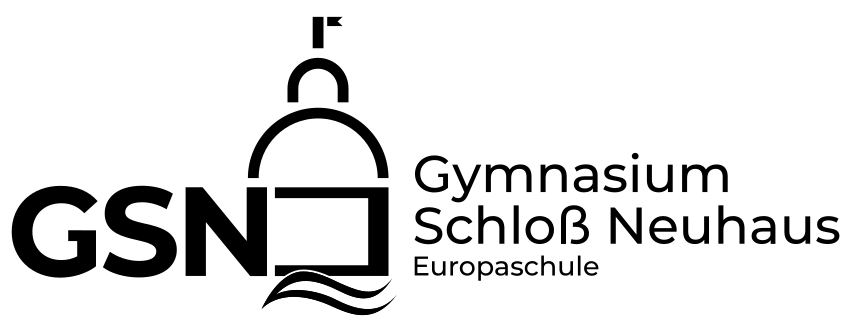
\includegraphics[width=10cm]{figures/example.png}
    \caption{Beispielbild mit Fußnote (\cite[Vgl.][465]{my-unique-book-id})}
    \label{fig:example}
\end{figure}

%\input{chapters/chapter3.tex}
%\input{chapters/chapter4.tex}
%\newpage
\section{Fazit}

\blindtext


\newpage
\begin{appendix}
  \addcontentsline{toc}{section}{Literaturverzeichnis}
  \printbibliography
  \newpage
  \addcontentsline{toc}{section}{Abbildungsverzeichnis}
  \listoffigures
  \newpage
  \addcontentsline{toc}{section}{Erklärung}
  {\protect\thispagestyle{empty}}
  \pagenumbering{gobble}
  Erklärung\\
\\
Hiermit erkläre ich, dass ich die vorliegende Arbeit selbstständig und ohne fremde Hilfe verfasst und keine anderen Hilfsmittel als die angegebenen Hilfsmittel verwendet habe. 
Insbesondere versichere ich, dass ich alle wörtlichen und sinngemäßen Übernahmen aus anderen Werken als solche kenntlich gemacht habe. 

\vspace{50pt}
\noindent\line(1,0){200} \hfill \line(1,0){200}\\
\noindent Datum, Ort \hfill Unterschrift
\end{appendix}

\end{document}
